\chapter{Experiments}

Having established our experimental setup and the environments we use, we move on to the experiments themselves. 
Firstly, we establish the benchmark scores for spectrograms, filterbanks and MFCCs.
Thereafter, we evaluate the quality of a single feature map obtained through the VGG16 network on both spectrograms and filterbanks as input, as well as examine the qualitative properties of the top feature maps.
Finally, we combine the top features obtained to form a hybrid feature map and evaluate the quality of these combined feature maps.

\section{Benchmark Scores}

In order to compare the quality of our newly acquired features, we need a benchmark score to compare it against. 
As stated in previous chapters, we use the AP scores obtained from the generic spectrograms, filterbanks and MFCCs of the Buckeye Corpus. 
Running the evaluation algorithm described in Chapter~\ref{chap:evaluation} on these features resulted in the AP scores shown in Table~\ref{tbl:benchmarks} and the precision-recall curves shown in Figure~\ref{fig:pr-curve}.

\begin{table}[!h]
    \mytable
    \caption{Benchmark AP scores for Spectrograms, filterbanks and MFCCs.}
    \begin{tabularx}{0.85\linewidth}{@{}lCC@{}}
        \toprule
        Feature         & & AP \\
        \midrule
        Spectrograms    & & $0.001038$ \\
        Filterbanks     & & $0.1890$ \\
        MFCCs           & & $0.2843$ \\
        \bottomrule
    \end{tabularx}
    \label{tbl:benchmarks}
\end{table}

As expected, spectrograms result in the lowest possible AP score of 0.001038 due to the high variability caused by different speakers, tones, channels and acoustic conditions. 
Filterbanks result in a significant improvement on spectrograms with an AP score of 0.189 due to the reduced impact of frequency ranges that fall outside normal speech. 
MFCCs, with an AP score of 0.2843, further improve on filterbanks by removing much of the spectral noise found within filterbanks as well as added improvement through the use of the delta and delta-delta features.

To gain some insight into how similarity between two of the same words are represented within each of these features, Figure~\ref{fig:cost_matrix} shows the cost matrix between two spoken phrases of the word "Graduate" calculated during Algorithm~\ref{alg:dtw} for spectrograms, filterbanks and MFCCs respectively. 
The DTW algorithm tries to find a minimum cost path from the top left of the cost matrix to the bottom right. 
As can be seen from the matrices, spectrograms have barely any similarity by the time it reaches the bottom right corner, hitting the upper cost limit about two thirds down.
Filterbanks, though they don't provide any natural path, end up with a fairly low cost point, but MFCCs can clearly be seen to be superior, with a natural flow of cost throughout the matrix as well as a lower endpoint.
This natural flow shows that MFCCs provide a consistent cost matrix for two phrases of the same word, and are a superior feature to spectrograms and filterbanks.

\begin{figure}[ht]
    \centering
    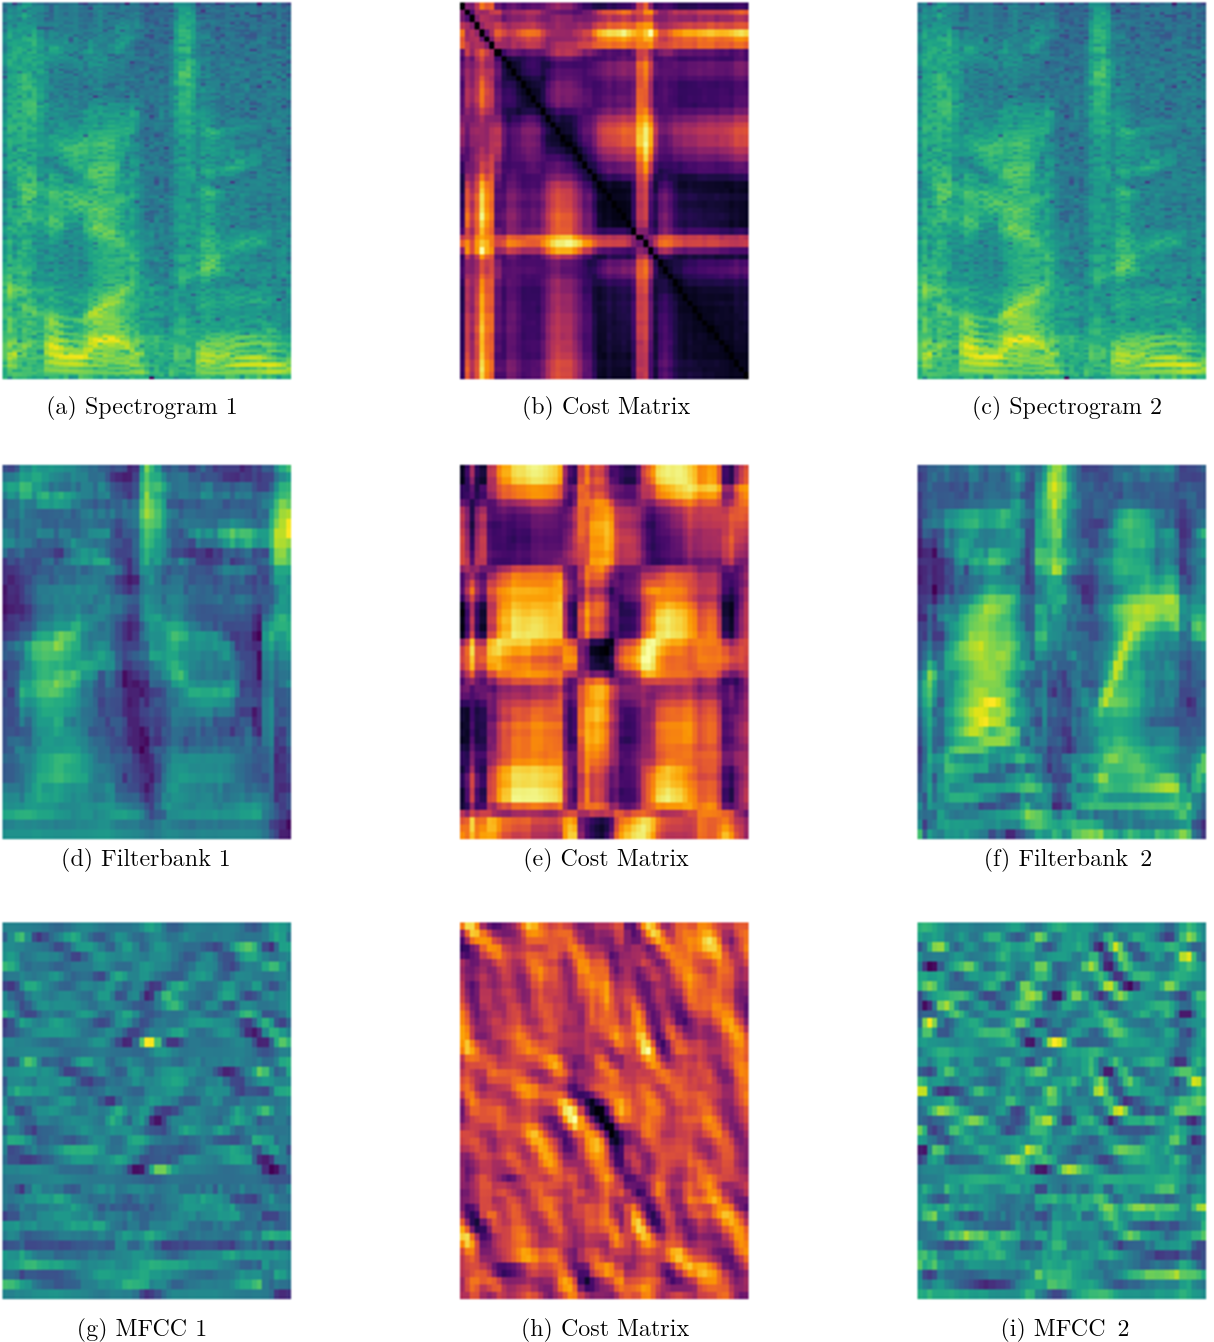
\includegraphics[width=0.6\linewidth]{content/fig/cost_matrices.png}
    \caption{Spectrogram, filterbank and MFCC for two spoken phrases of the word "graduate" and the cost matrix between each, with lighter colour representing a lower cost.}
    \label{fig:cost_matrix}
\end{figure}

\section{Single Filter Analysis}

Now that our benchmark has been set, we move on to our first experiment to evaluate the features per individual feature map obtained from the VGG16 network. 
We obtain these features from two input features, namely the spectrograms and the filterbanks.
With the features obtained from the spectrogram we at the very least hope to improve our AP score relative to that of the spectrogram benchmark score, and with those derived from the filterbanks we hope to not only improve on the benchmark filterbank score, but also on the MFCC score, thereby improving on existing feature extraction techniques as well as possibly reducing the input vector size.

\subsection{Spectrogram Filters}

Evaluate filters when applied to spectrograms, can be subdivided into layers

\subsection{Filterbank Filters}

Evaluate filters when applied to filterbanks, can be subdivided into layers

\section{Combined Filter Analysis}

Using the top performing filters and combining them, then get AP scores.
(Perhaps go into qualitative analysis for top filters)

\subsection{Top Spectrogram Filters}

\subsection{Top Filterbank Filters}

\subsection{Top Combined Filters}

\section{Summary of Results}

Show summarised results table with final, top performing feature set.